\section{Implementation}

%\subsection{Processes}

\begin{figure}[!b]
	\centering
	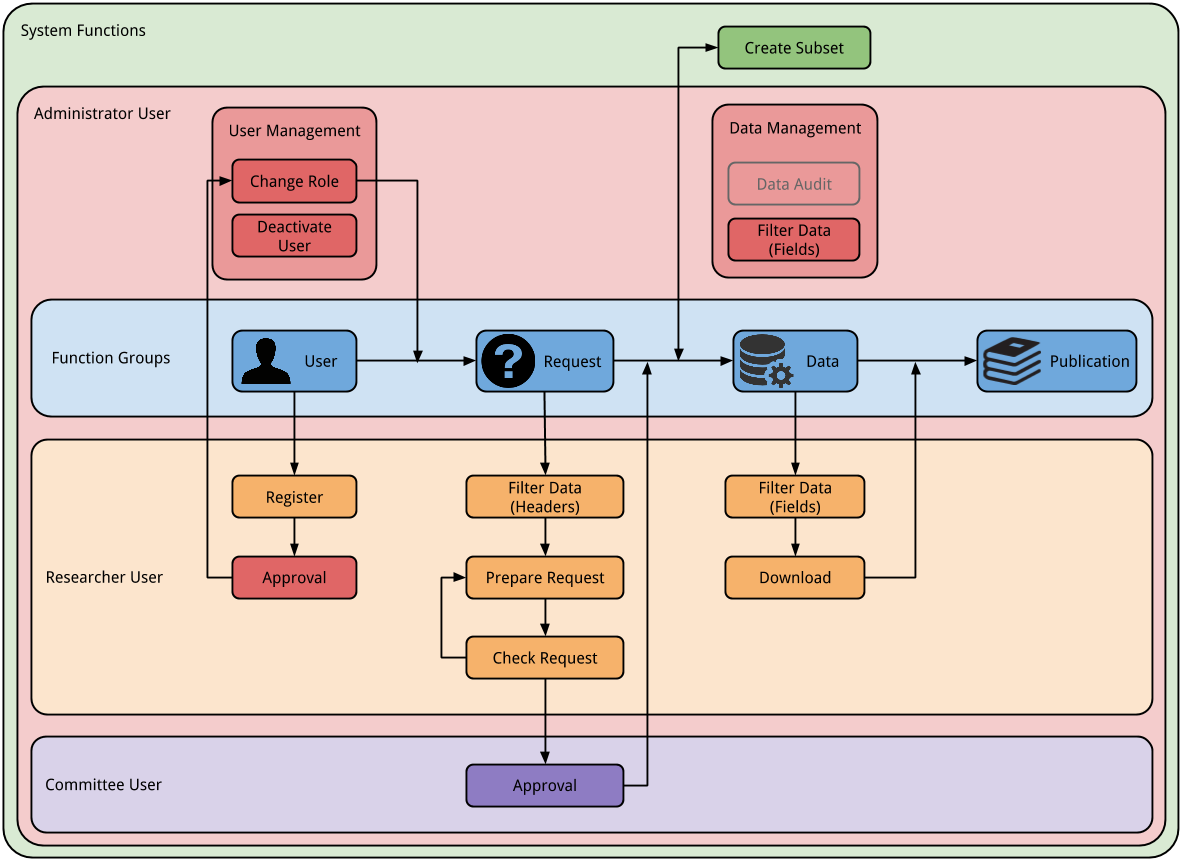
\includegraphics[width=1.0\linewidth]{images/functions-implemented}
	\caption{
		Mapping of functions after implementation considerations according to function groups, actors, and research workflow.
		Greyed-out functions are implemented through place holders. \silvia{so they are not in prototype? and what is the difference between this and 3.1?}
	}
	\label{fig:functions-implemented}
\end{figure}


%\paragraph{Division of management tasks}
Due to time restrictions in this study not all functions that were discovered in chapter 2 can be implemented.
\silvia{do you know the package clever references? cleverref - if not, ask Shayan ;-) }
A selection is made based on the programmers opinion what would be most profitable for a prototype system.
The selection that is made can be seen in figure \ref{fig:functions-implemented}.
Decisions are based on the fact that the demo has to appeal to a wide variety of users, most importantly research and clinic management.

\silvia{i stopped here for now, will continue later tonight}
To start with the most basic system data management functions are implemented.
These include search and filtering for the researcher user and data manager user, and the download function.
Data audit is implemented through placeholders to show the value of such an function without the actual data processing back-end.
Metadata handling is not implemented as data is considered \emph{fixed} after system initialisation.

After this, request management is implemented.
Removing direct access to data and adding more control for committee users (coming directly from each clinic) is deemed to increase system trust by clinic management.
Request creation, editing, and submission by researcher users is supported.
Approval by committee users and automated subset creation by the system is also implemented.
Not implemented are: annotation and feedback on requests, stale request detection, and keeping provenance.
All of these functions are mostly supporting users in performing tasks but are not critical to the execution of the system.

User management is implemented with the addition of roles to user accounts and a dashboard for the data manager user.
In this dashboard the manager can find all the users of the system and assign the appropriate roles to each of them.
Lastly, publication management as closing stone of the research cycle is left out.
At this moment the additional time that has to be spend including these functions does not outweigh the added value for prospective demo users.

\paragraph{Security}
Even though security considerations are a big part of the requirement analysis (see section \ref{security}), it does not show itself that clearly in the system implementation.
Most of the security measures were taken during the data gathering steps.
Because the decision was made to have a fixed dataset for the system a lot of the discussed security measures do not need to apply anymore as described in section \ref{security-summarisation-analysis}.

Provenance, as part of security, was not implemented either.
It would be very useful to show the strength of the \ivfsystem{}, data protection through provenance can be made highly visible and easy to understand for humans.
However, the goals to quickly support the provenance functions and develop an interface on top of the data could not be reached within the time frame.

Lastly, in order to obtain a working system a few more things are needed.
More functionality needs to be implemented, most notably better user interfaces for data filtering and selection (see section \ref{evaluation}).
Furthermore, more design and programming iterations need to be done before the request and publication management have been fully developed.
Then a big security iteration should be done to prepare the system for testing and certification.
Right now security has been patched up in the front-end by hiding information for certain users, this should change to the back-end not \emph{providing} that information to begin with.